%-------------------------------------------
\begin{frame}[containsverbatim]
\frametitle{Practical exercise}
%-------------------------------------------
\begin{exampleblock}{}
For this practical exercise on Snakemake we will:
\begin{itemize}
    \item access to snakemake by the way of a docker container
    \item access to analysis tools by the way of a conda environment (details about conda will be seen after)
    \item create a first snakefile with one rule
    \item add a second rule to create the first workflow
\end{itemize}
During this first exercise, we will execute several cycles: executing snakemake, observing the result and improving the code. Each code version will be noted \verb|ex1_oX.smk| with X a progressive digit.
\end{exampleblock}
\end{frame}
%-------------------------------------------
\begin{frame}[containsverbatim]
\frametitle{Exercise setup}
%-------------------------------------------
We will access to Snakemake by running a docker image containing the conda tool (among other):
\begin{exampleblock}{docker miniconda3 (git 2.20.1 + conda 4.8.2)}
\begin{lstlisting}
docker run -i -t -v ${PWD}:/data continuumio/miniconda3
\end{lstlisting}
\end{exampleblock}

%\begin{exampleblock}{docker from NBIS courses (conda 4.6.14 + git 2.7.4)}
%\begin{lstlisting}
%sudo docker run -it -p 8888:8888 -v ${PWD}:/course/ scilifelablts/reproducible_research_course_slim
%\end{lstlisting}
%\end{exampleblock}

\begin{exampleblock}{Conda environment}
And, we will access to the analysis tools thanks to a conda environment, \verb|envfair.yml| (cf. next slide), designed for this exercise:
\begin{lstlisting}
conda env create -n envfair -f envfair.yml
conda activate envfair
\end{lstlisting}
\end{exampleblock}
\end{frame}
%-------------------------------------------
\begin{frame}[containsverbatim]
\frametitle{Exercise setup}
%-------------------------------------------
\begin{exampleblock}{envfair.yml}
\begin{lstlisting}[language=python]
channels:
  - conda-forge
  - bioconda
  - main
  - default
dependencies:
  - python=3.7.6 # specify python version (not required but can help with downstream conflicts)
  - snakemake-minimal=5.10.0 # workflow manager
  - graphviz=2.42.3 # for visualisation
  - xorg-libxrender
  - xorg-libxpm
  - wget=1.20.1 # for downloading files
  - fastqc=0.11.9 # for the RNAseq analysis
  - bowtie2=2.4.1
  - samtools=1.10
  - subread=2.0.1
\end{lstlisting}
\end{exampleblock}
\end{frame}
%-------------------------------------------
\begin{frame}[containsverbatim]
\frametitle{Rule concept with one input file}
%-------------------------------------------
\begin{exampleblock}{Objective 1}
Create a snakemake file named \verb|ex1_o1.smk| including the first step of the RNAseq workflow (the reads quality checking thank to the \verb|fastqc| tool) on one of the RNAseq files
\end{exampleblock}
\begin{exampleblock}{Hint}
\begin{itemize}
    \item input file: \verb|SRR3099585_chr18.fastq.gz| in a local directory of yours
    \item fastqc access: by running \verb|docker miniconda3| + activate the conda \verb|envfair| environment
    \item fastqc command: \verb|fastqc inputFileName --outdir ResultDirectory|
    \item the 2 fastqc result files (.zip $\&$ .html) are named based on the prefix of input file
\end{itemize}
\end{exampleblock}
\end{frame}
%-----------------------------------------------
\begin{frame}[containsverbatim]
\frametitle{Solution}
%-------------------------------------------
% biocontainers/fastqc ne fonctionne pas 
% (malgré les +50k download et maj 2 mois):
% - pas de version latest, obligation de spécifier le tag v0.11.9_cv6 (cv5 ne fonctionne pas non plus)
% choix pegi3s/fastqc qui est mieux documenté (mais maj 5 mois)
\begin{exampleblock}{ex1$\_$o1.smk}
\begin{lstlisting}[language=python]
rule fastqc:
  output:
    "FastQC/SRR3099585_chr18_fastqc.zip", 
    "FastQC/SRR3099585_chr18_fastqc.html"
  input:
    "Data/SRR3099585_chr18.fastq.gz"
  shell: "fastqc --outdir FastQC/ {input}"
\end{lstlisting}
\end{exampleblock}
\begin{exampleblock}{Snakemake run}
\begin{lstlisting}[language=python]
snakemake --snakefile ex1_o1.smk
\end{lstlisting}
\end{exampleblock}
\begin{exampleblock}{Observe result}
Look at the newly created \verb|FastQC| directory: Snakemake create needed directories.
\end{exampleblock}
\end{frame}
%-------------------------------------------
\begin{frame}[containsverbatim]
\frametitle{One rule, 2 input files}
%-------------------------------------------
\begin{exampleblock}{Objective 2}
Add a second input RNAseq file to the rule
\end{exampleblock}
\begin{exampleblock}{Hint}
\begin{itemize}
    \item input file: \verb|SRR3099586_chr18.fastq.gz| in a local directory of yours
\end{itemize}
\end{exampleblock}
\end{frame}
%-----------------------------------------------
\begin{frame}[containsverbatim]
\frametitle{Solution}
%-------------------------------------------
\begin{exampleblock}{ex1$\_$o2.smk}
\begin{lstlisting}[language=python]
rule fastqc:
  output:
    "FastQC/SRR3099585_chr18_fastqc.zip", 
    "FastQC/SRR3099585_chr18_fastqc.html",
    "FastQC/SRR3099586_chr18_fastqc.zip", 
    "FastQC/SRR3099586_chr18_fastqc.html"
  input:
    "Data/SRR3099585_chr18.fastq.gz",
    "Data/SRR3099586_chr18.fastq.gz"
  shell: "fastqc --outdir FastQC/ {input}"
\end{lstlisting}
\end{exampleblock}
\begin{exampleblock}{Snakemake run}
\begin{lstlisting}[language=python]
# -s is the short form of the --snakefile option
snakemake -s ex1_o2.smk
\end{lstlisting}
\end{exampleblock}
\end{frame}
%-------------------------------------------
\begin{frame}[containsverbatim]
\frametitle{Solution}
%-------------------------------------------
\begin{exampleblock}{Observe result}
Why does Snakemake reply \verb|"Nothing to be done"|?\\
Two solutions:\begin{itemize}
\item delete the FastQC directory (\verb|rm -Rf FastQC|) and rerun the snakemake command
\item use the Snakemake \verb|--forcerules| (\verb|-R|) option: \verb|snakemake -s ex1_o2.smk -R fastqc|
\end{itemize}
\end{exampleblock}
\end{frame}
%-------------------------------------------
\begin{frame}[containsverbatim]
\frametitle{Manage all the RNAseq files}
%-------------------------------------------
\begin{exampleblock}{Objective 3}
Add all the RNAseq files.\\
Boring with writing all input and output file names? \\
Use the \verb|expand()| function to manage all the input RNAseq files at once.
\end{exampleblock}
\begin{exampleblock}{Hint}
\begin{itemize}
    \item create a Python list at the begining of the snakefile and containing all the basename of the input files (don't include the "\verb|.fastq.gz|" suffix).\\
    Python list: \verb|list_name = ["item1", "item2", ..., "itemN"]|
    \item replace the filename lists of the input and output directives by the \verb|expand()| function
\end{itemize}
\end{exampleblock}
\end{frame}
%-----------------------------------------------
\begin{frame}[containsverbatim]
\frametitle{Solution}
%-------------------------------------------
\begin{exampleblock}{ex1$\_$o3.smk}
\begin{lstlisting}[language=python]
SAMPLES = ["SRR3099585_chr18","SRR3099586_chr18","SRR3099587_chr18"] # add others samples

rule fastqc:
  output:
    expand("FastQC/{sample}_fastqc.zip", sample = SAMPLES),
    expand("FastQC/{sample}_fastqc.html", sample = SAMPLES)
  input:
    expand("Data/{sample}.fastq.gz", sample = SAMPLES)
  shell: "fastqc --outdir FastQC/ {input}"
\end{lstlisting}
\end{exampleblock}
\begin{exampleblock}{Snakemake run}
\begin{lstlisting}[language=python]
rm -Rf FastQC/
snakemake -s ex1_o3.smk
\end{lstlisting}
\end{exampleblock}
\end{frame}
%-----------------------------------------------
\begin{frame}[containsverbatim]
\frametitle{Add a second rule}
%-----------------------------------------------
\begin{exampleblock}{Objective 4}
Add a second rule, this will start a workflow. \\
The second rule concerns the creation of an index file for the genome sequence (needed for the mapping step). As the mapping tool is bowtie2, the index creation tool is bowtie2-build.
\end{exampleblock}
\begin{exampleblock}{Hint}
\begin{itemize}
    \item genome file (input): \verb|Data/O.tauri_genome.fna|
    \item use a Python list and the \verb|expand()| function to manage the 6 index files names that will be created by the command: "*.1.bt2" ... "*.4.bt2","*.rev.1.bt2","*.rev.2.bt2"
    \item command: \verb|bowtie2-build genomeSequenceAccess indexAccessPrefix|
\end{itemize}
\end{exampleblock}
\end{frame}
%-----------------------------------------------
\begin{frame}[containsverbatim]
\frametitle{Solution}
%-------------------------------------------
\begin{exampleblock}{ex1$\_$o4.smk (copy, run)}
\begin{lstlisting}[language=python]
SAMPLES = ["SRR3099585_chr18","SRR3099586_chr18","SRR3099587_chr18"]
BIDX = ["1","2","3","4","rev.1","rev.2"]

rule genome_bwt2_index:
  output:
    expand("Tmp/Otauri.{ext}.bt2", ext=BIDX)
  input:
    "Data/O.tauri_genome.fna"
  shell: "bowtie2-build {input} Tmp/Otauri"

rule fastqc:
  output:
    expand("FastQC/{sample}_fastqc.zip", sample = SAMPLES),
    expand("FastQC/{sample}_fastqc.html", sample = SAMPLES)
  input:
    expand("Data/{sample}.fastq.gz", sample = SAMPLES)
  shell: "fastqc --outdir FastQC/ {input}"
\end{lstlisting}
\end{exampleblock}
%\begin{exampleblock}{Snakemake run}
%\begin{lstlisting}[language=python]
%snakemake -s ex1_o4.smk
%\end{lstlisting}
%\end{exampleblock}
\end{frame}
%-------------------------------------------
\begin{frame}[containsverbatim]
\frametitle{Solution}
%-------------------------------------------
\begin{exampleblock}{Observe result}
Does Snakemake do the job?\\
Why wasn't the fastqc command launched?\\
\end{exampleblock}
\begin{exampleblock}{rule links}
Snakemake run the first rule and stop when the target files are present. Also, there is no link between the 2 rules because they concern two independent parts of the analysis.\\
The solution is to add a rule that aggregate this 2 parts of the workflow.
\end{exampleblock}
\end{frame}
%-------------------------------------------
\begin{frame}[containsverbatim]
\frametitle{The target rule}
%-------------------------------------------
\begin{exampleblock}{Objective 5}
Add a "first" rule (rule all, target, ...) with the expected results for the 2 rules (\verb|fastqc| and \verb|genome_bwt2_index| in its \verb|input:| directive.
\end{exampleblock}
\end{frame}
%-------------------------------------------
\begin{frame}[containsverbatim]
\frametitle{Solution}
%-------------------------------------------
\begin{exampleblock}{ex1$\_$o5.smk}
\begin{lstlisting}
...

rule all:
  input:
    expand("FastQC/{sample}_fastqc.html", sample=SAMPLES),
    expand("Tmp/Otauri.{ext}.bt2", ext=BIDX)

...
\end{lstlisting}
\end{exampleblock}
\begin{exampleblock}{Snakemake run}
\begin{lstlisting}[language=python]
snakemake -s ex1_o5.smk -R all fastqc
\end{lstlisting}
\end{exampleblock}
\end{frame}
%-------------------------------------------
\begin{frame}[containsverbatim]
\frametitle{Solution}
%-------------------------------------------
\begin{exampleblock}{Observe result}
Does Snakemake do the job?\\
\end{exampleblock}
\begin{exampleblock}{Fastqc: job or jobs?}
Look at more precisely the fastqc job. We have many input files but snakemake launched only one fastqc job:
\begin{center}
    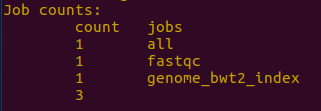
\includegraphics[width=6cm]{03_workflow/images/FAIR_ex1_o5_smk.png}
\end{center}
It is because the \verb|fastqc| rule is defined with a list of files and not for one unique file and because the \verb|fastqc| tool accepts both a unique file as well as a list of files.
\end{exampleblock}
\end{frame}
%-------------------------------------------
\begin{frame}[containsverbatim]
\frametitle{Running n individual jobs}
%-------------------------------------------
\begin{exampleblock}{Objective 6}
Thank to the \verb|all| rule, all expected files are designated. So we don't need to give the \verb|fastqc| rule a list anymore and we can replace it to manage only one file and all files one by one. We will gain in power in systems having more than one core.
\end{exampleblock}
\begin{exampleblock}{Hint}
Replace the \verb|expand()| function with a wildcard for one filename in the \verb|fastqc| rule.
\end{exampleblock}
\end{frame}
%-------------------------------------------
\begin{frame}[containsverbatim]
\frametitle{Solution}
%-------------------------------------------
\begin{exampleblock}{ex1$\_$o6.smk}
\begin{lstlisting}
rule fastqc:
  output:
    "FastQC/{sample}_fastqc.zip",
    "FastQC/{sample}_fastqc.html"
  input:
    "Data/{sample}.fastq.gz"
  shell: "fastqc --outdir FastQC/ {input}"
\end{lstlisting}
\end{exampleblock}
\begin{exampleblock}{Snakemake run}
\begin{lstlisting}[language=python]
snakemake -s ex1_o6.smk -R all fastqc
\end{lstlisting}
\end{exampleblock}
\end{frame}
%-------------------------------------------
\begin{frame}[containsverbatim]
\frametitle{Solution}
%-------------------------------------------

\begin{exampleblock}{Observe result}
Now Snakemake did many fastqc jobs:
\begin{center}
    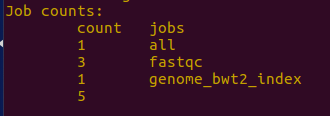
\includegraphics[width=6cm]{03_workflow/images/FAIR_ex1_o6_smk.png}
\end{center}
But what happens to the runtime displays on the screen?\\

To correct this, we will move the displays to a log file specific for each rule and each input file.
\end{exampleblock}
\end{frame}
%-------------------------------------------
\begin{frame}[containsverbatim]
\frametitle{Adding log file}
%-------------------------------------------
\begin{exampleblock}{Objective 7}
In Unix systems, the output of a command is usually sent to two separate streams: the normal output: to Standard Out (stdout also "\verb|>|" in shell), and error messages: to Standard Error (stderr, or "\verb|2>|" in shell). To integrate stderr into the same log file as the stdout can be use "\verb|&>|" instead of "\verb|>|": \\ 
shell: ...  \verb|&> {log}|", but use with care when output files are printed to stdout (as often in shell comands).\\
Redirect the stdout and stderr streams of the \verb|fastqc| and bowtie2-build commands. \\
\end{exampleblock}
\begin{exampleblock}{Hint}
For the \verb|bowtie2-build| and \verb|fastqc| rules, add the \verb|log:| directive with two variables (\verb|log1| and \verb|log2|) to redirect each streams.
\end{exampleblock}
\end{frame}
%-----------------------------------------------
\begin{frame}[containsverbatim]
\frametitle{Solution}
%-------------------------------------------
\begin{exampleblock}{ex1$\_$o7.smk}
\begin{lstlisting}[language=python]
# in rule genome_bwt2_index:
  log:
    log1="Logs/genome_bwt2_index.log1",
    log2="Logs/genome_bwt2_index.log2"
  shell: "bowtie2-build {input} Tmp/Otauri 1>{log.log1} 2>{log.log2}"
# in rule fastqc:
  log:
    log1="Logs/{sample}_fastqc.log1",
    log2="Logs/{sample}_fastqc.log2"
  shell: "fastqc --outdir FastQC/ {input} 1>{log.log1} 2>{log.log2}"
\end{lstlisting}
\end{exampleblock}
\begin{exampleblock}{Snakemake run}
\begin{lstlisting}[language=python]
rm -Rf FastQC/ Tmp/ Logs/; snakemake -s ex1_o7.smk
\end{lstlisting}
\end{exampleblock}
\end{frame}